\element{PFSStrat}{
\begin{questionmult}{pfsstrat 01a}
Soit le modèle suivant. On cherche, en statique, la relation entre le couple moteur, la pesanteur et le ressort. 
On cherche à savoir quelle pièce, ou quel ensemble de pièces commencer par isoler. 
\begin{center}
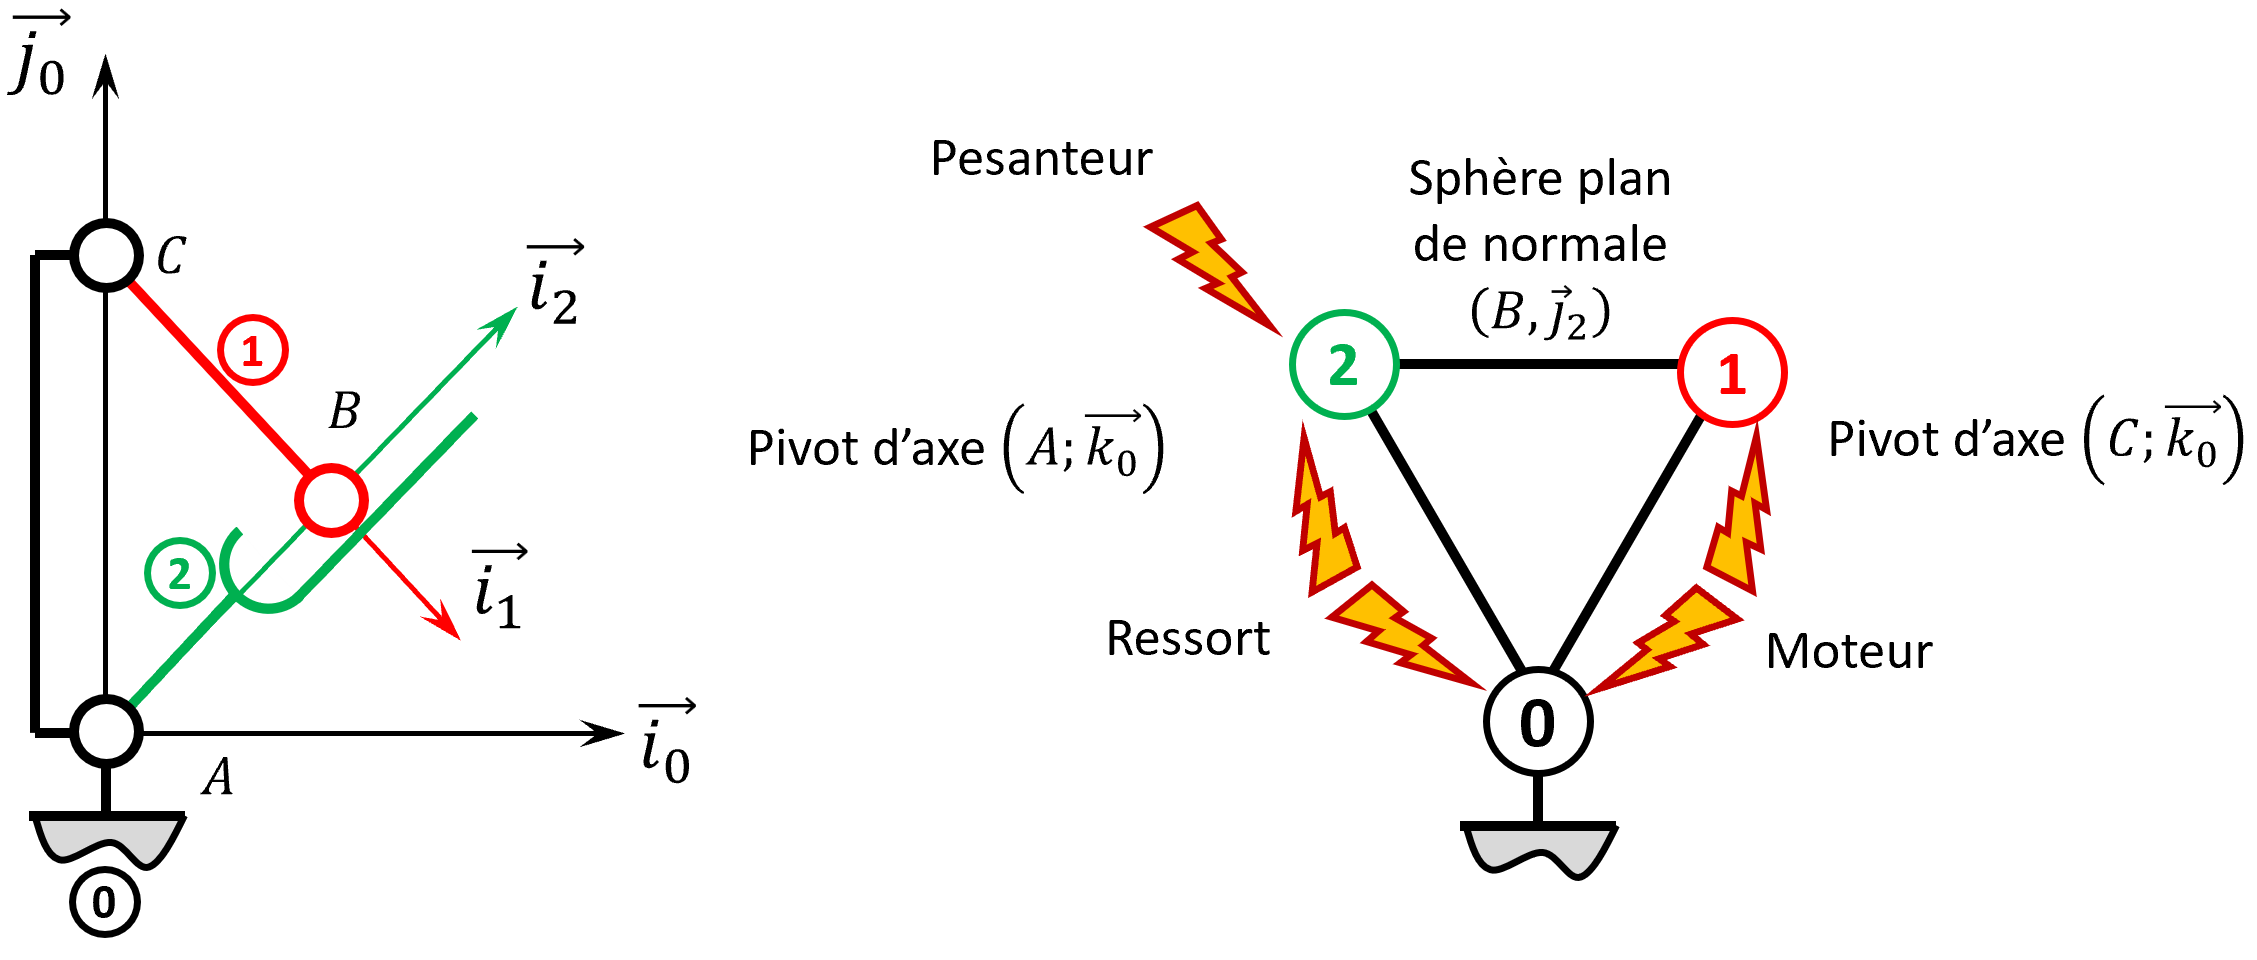
\includegraphics[width=.95\linewidth]{pfs_strategie_sympact_01}
\end{center}
	\begin{reponses}	
	\bonne {Peu importe.}
	\mauvaise {On commence par isoler 0.}
	\mauvaise {On commence par isoler 1.} 
	\mauvaise {On commence par isoler 2.}
	\mauvaise {On commence par isoler 1+2.}
	\end{reponses}
\end{questionmult}\\}

\element{PFSStrat}{
\begin{questionmult}{pfsstrat 01b}
Soit le modèle suivant. On cherche, en statique, la relation entre le couple moteur, la pesanteur et le ressort. 
On a isolé 1. Quelle équation est-il intéressante d'écrire ?
\begin{center}
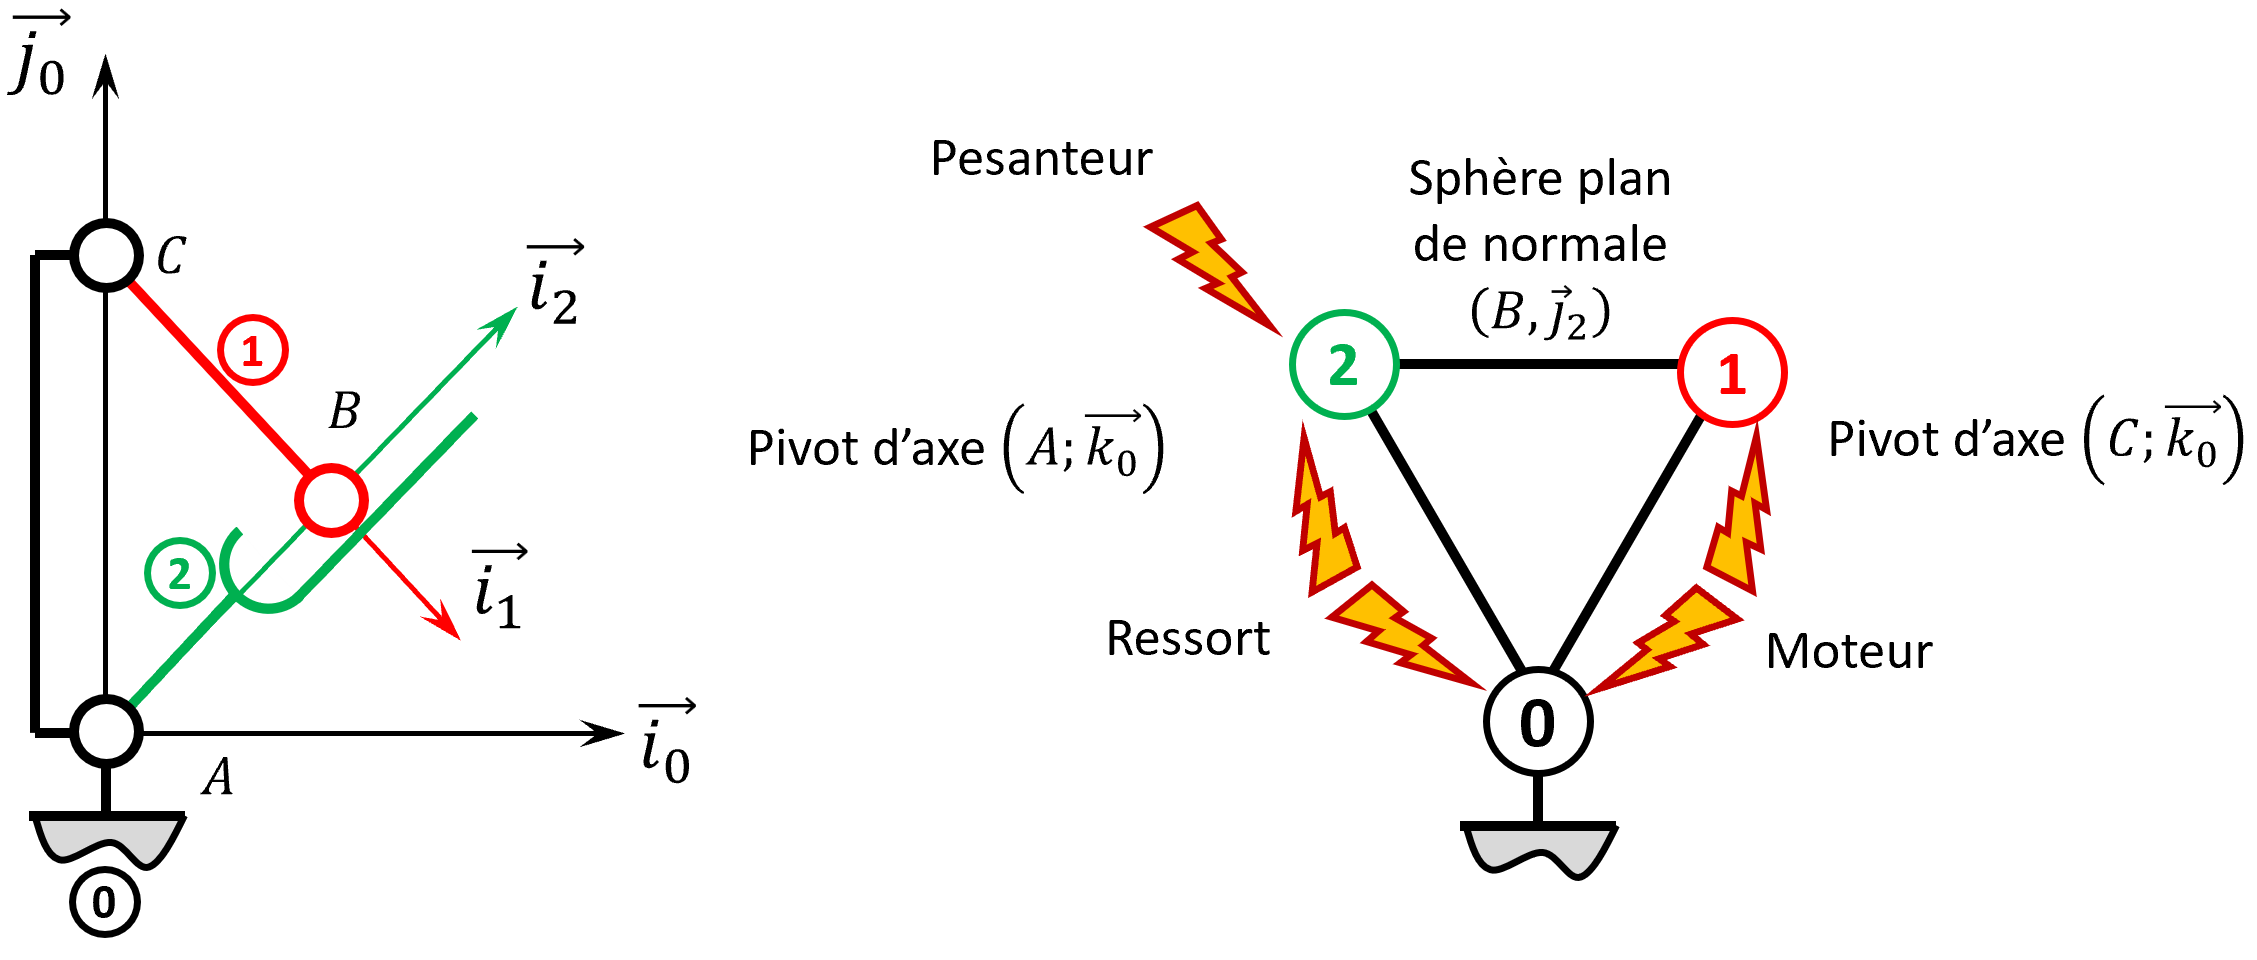
\includegraphics[width=.95\linewidth]{pfs_strategie_sympact_01}
\end{center}
	\begin{reponses}	
	\bonne {le TMS.}
	\mauvaise {le TRS.}
	\mauvaise {le PFS.}
	\mauvaise {en $A$.}
	\mauvaise {en $B$.}
	\bonne {en $C$.}
	\mauvaise {en projection sur $\vi{0}$.}
	\mauvaise {en projection sur $\vj{0}$.}		
	\mauvaise {en projection sur $\vi{1}$.}
	\mauvaise {en projection sur $\vj{1}$.}		
	\mauvaise {en projection sur $\vi{2}$.}
	\mauvaise {en projection sur $\vj{2}$.}		
	\bonne {en projection sur $\vz{0}$.}	
		\mauvaise {ce n'est pas la meilleure idée.}
	\end{reponses}
\end{questionmult}\\}

\element{PFSStrat}{
\begin{questionmult}{pfsstrat 01c}
Soit le modèle suivant. On cherche, en statique, la relation entre le couple moteur, la pesanteur et le ressort. 
On a isolé 2. Quelle équation est-il intéressante d'écrire ?
\begin{center}
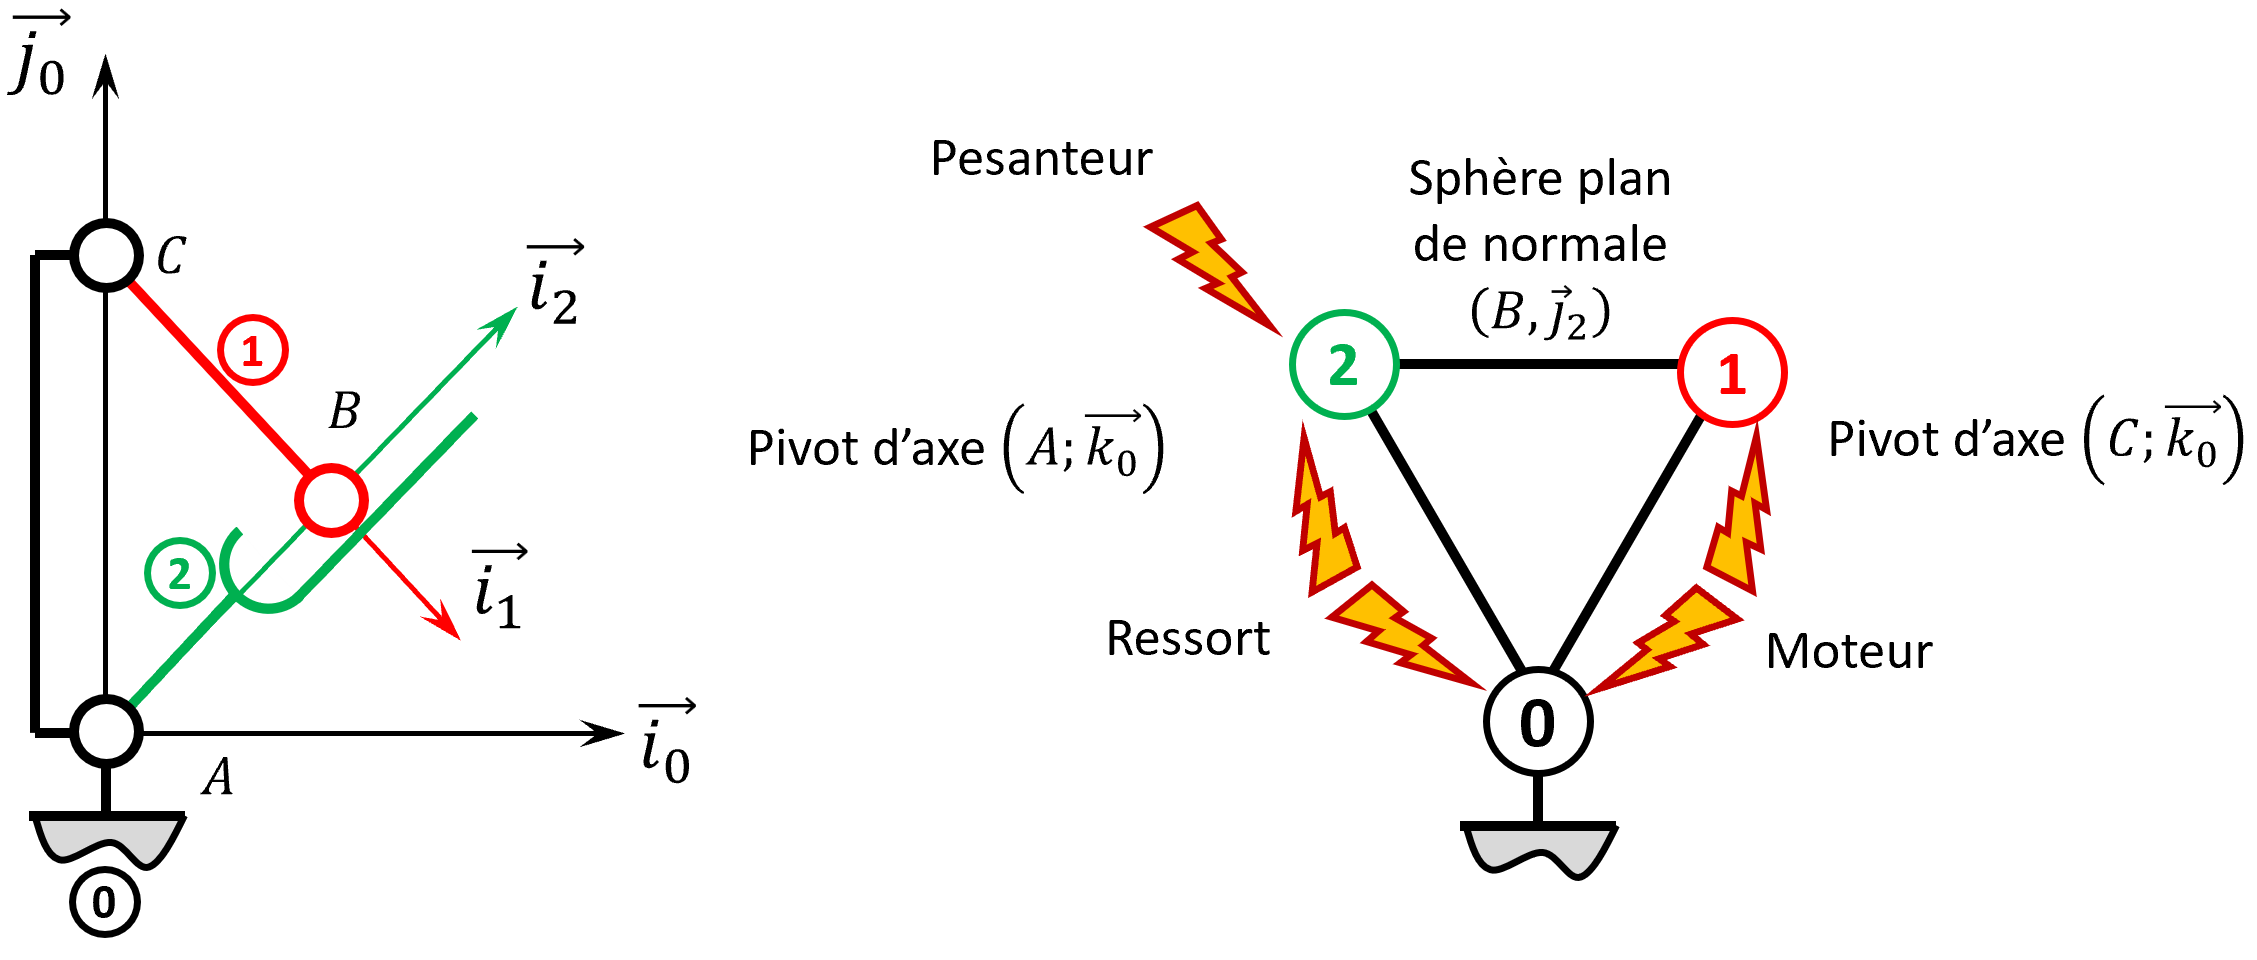
\includegraphics[width=.95\linewidth]{pfs_strategie_sympact_01}
\end{center}
	\begin{reponses}	
	\bonne {le TMS.}
	\mauvaise {le TRS.}
	\mauvaise {le PFS.}
	\bonne {en $A$.}
	\mauvaise {en $B$.}
	\mauvaise {en $C$.}
	\mauvaise {en projection sur $\vi{0}$.}
	\mauvaise {en projection sur $\vj{0}$.}		
	\mauvaise {en projection sur $\vi{1}$.}
	\mauvaise {en projection sur $\vj{1}$.}		
	\mauvaise {en projection sur $\vi{2}$.}
	\mauvaise {en projection sur $\vj{2}$.}		
	\bonne {en projection sur $\vz{0}$.}	
		\mauvaise {ce n'est pas la meilleure idée.}
	\end{reponses}
\end{questionmult}\\}


\element{PFSStrat}{
\begin{questionmult}{pfsstrat 02a}
Soit le modèle suivant. On cherche, en statique, la relation entre le poids du camion et l'effort extérieur.
\begin{center}
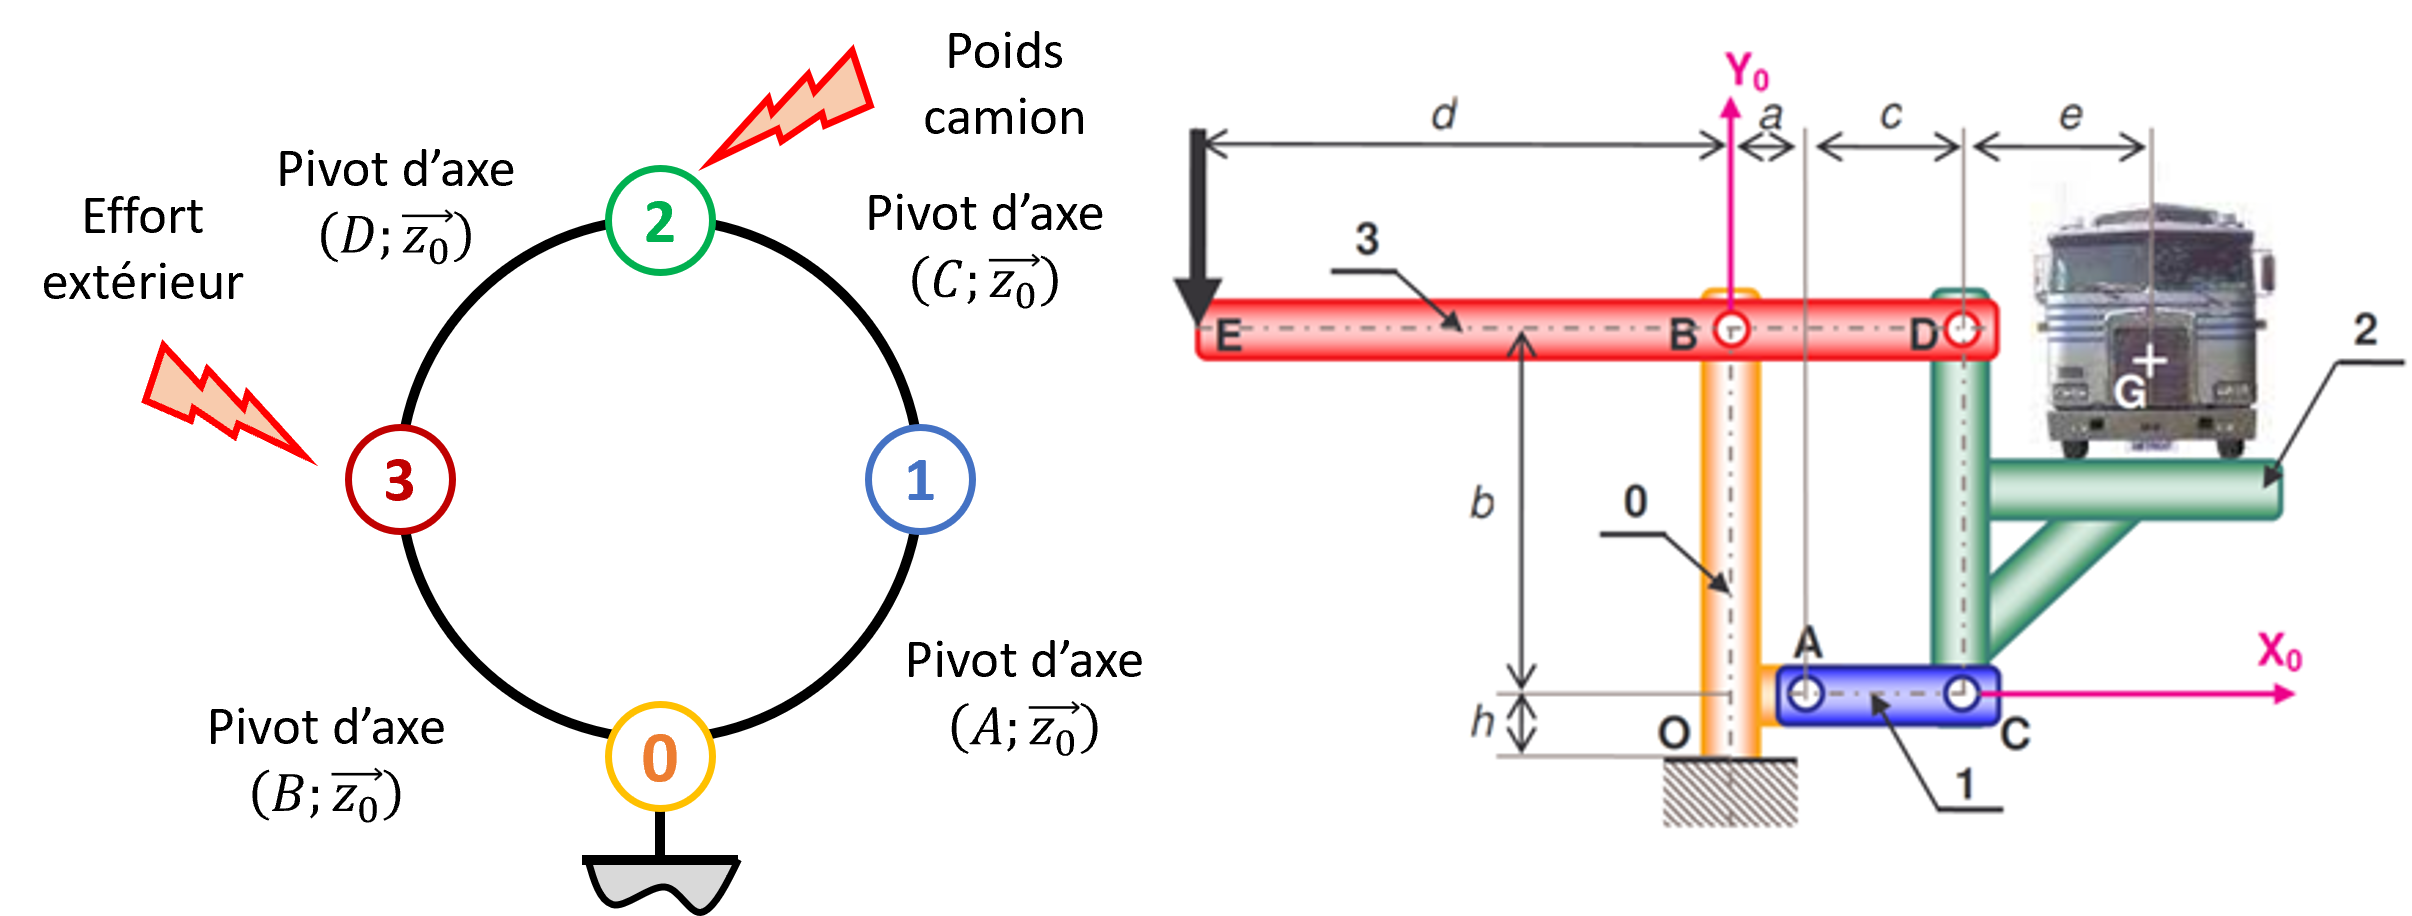
\includegraphics[width=.95\linewidth]{pfs_strategie_pese_camion}
\end{center}
	\begin{reponses}	
	\bonne{On commence par isoler 1.} 
	\mauvaise {Peu importe.}
	\mauvaise {On commence par isoler 1+2+3.} 
	\mauvaise {On commence par isoler 1+2+3.} 
	\mauvaise {On commence par isoler 1+2.} 
	\mauvaise {On commence par isoler 3+2.} 
	\mauvaise {On commence par isoler 3+1.} 
	\mauvaise {On commence par isoler 3.}
	\mauvaise {On commence par isoler 0.}
	\end{reponses}
\end{questionmult}\\}

\element{PFSStrat}{
\begin{questionmult}{pfsstrat 02b}
Soit le modèle suivant. On cherche, en statique, la relation entre le poids du camion et l'effort extérieur.
On a isolé 1. Quelle équation est-il préférable d'écrire ?
\begin{center}
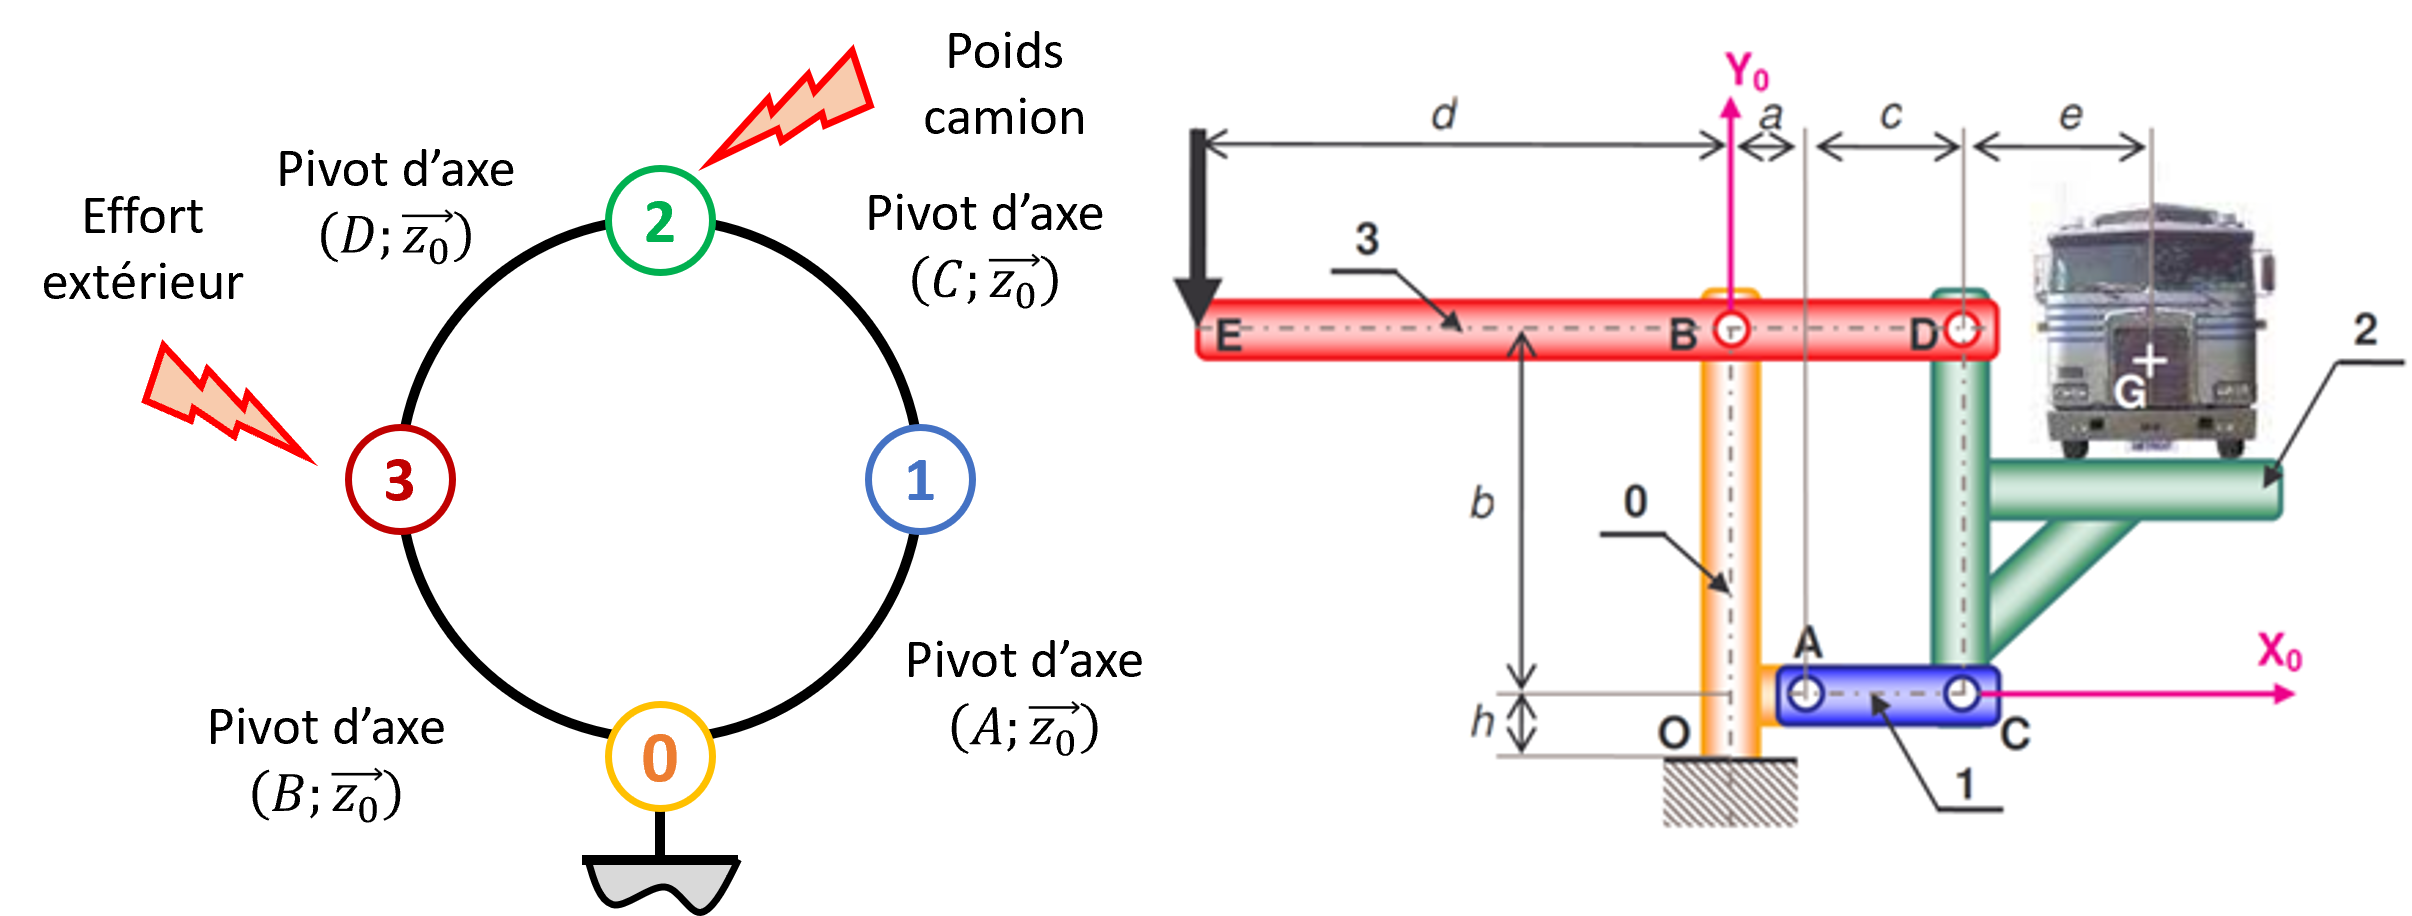
\includegraphics[width=.95\linewidth]{pfs_strategie_pese_camion}
\end{center}
	\begin{reponses}	
	\mauvaise {le TMS.}
	\mauvaise {le TRS.}
	\bonne {le PFS.}
	\mauvaise {en $A$.}
	\mauvaise {en $B$.}
	\mauvaise {en $C$.}
	\mauvaise {en $D$.}
	\mauvaise {en $E$.}
	\mauvaise {en projection sur $\vx{0}$.}
	\mauvaise {en projection sur $\vy{0}$.}		
	\mauvaise {en projection sur $\vz{0}$.}
		\mauvaise {ce n'est pas la meilleure idée.}
	\end{reponses}
\end{questionmult}\\}

\element{PFSStrat}{
\begin{questionmult}{pfsstrat 02c}
Soit le modèle suivant. On cherche, en statique, la relation entre le poids du camion et l'effort extérieur.
On a isolé 2. Quelle équation est-il préférable d'écrire ?
\begin{center}
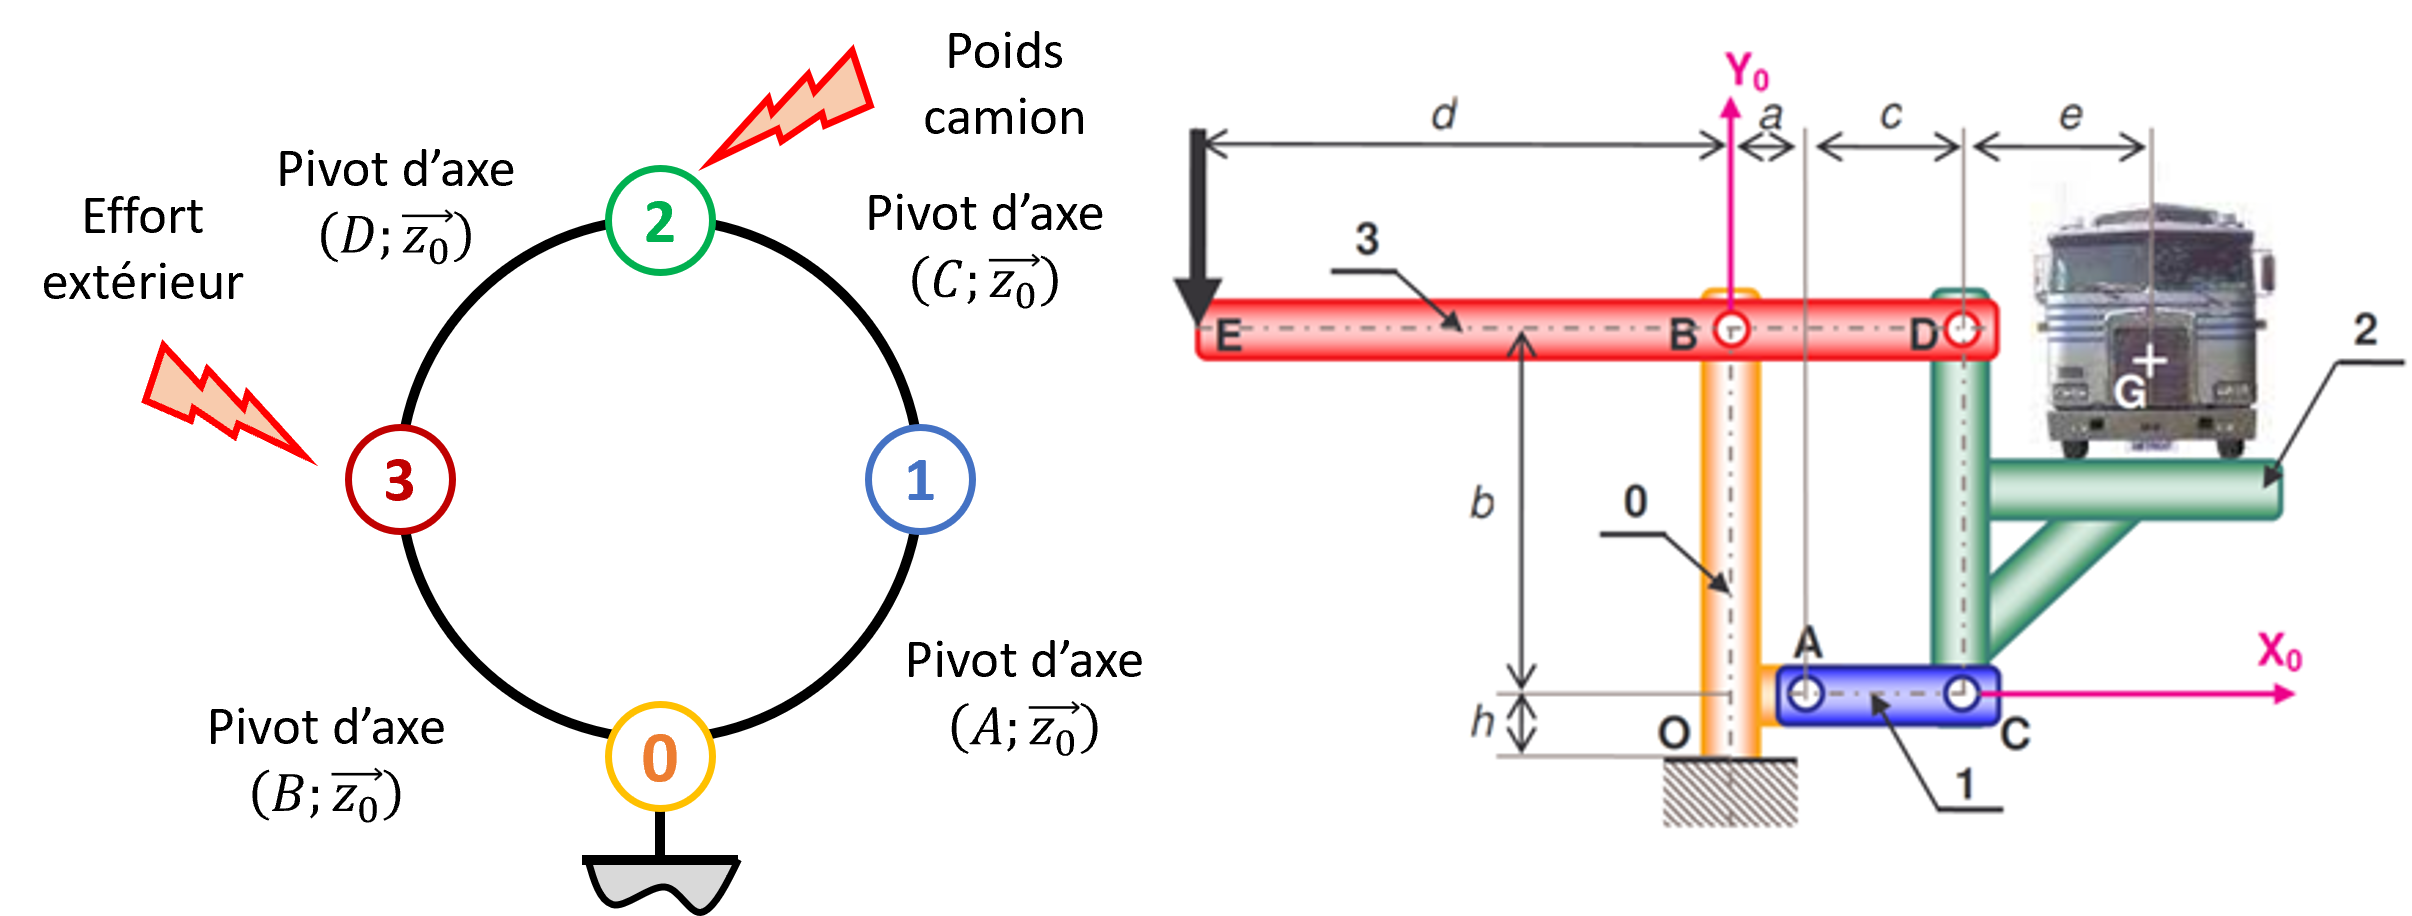
\includegraphics[width=.95\linewidth]{pfs_strategie_pese_camion}
\end{center}
	\begin{reponses}	
	\mauvaise {le TMS.}
	\bonne {le TRS.}
	\mauvaise {le PFS.}
	\mauvaise {en $A$.}
	\mauvaise {en $B$.}
	\mauvaise {en $C$.}
	\mauvaise {en $D$.}
	\mauvaise {en $E$.}
	\mauvaise {en projection sur $\vx{0}$.}
	\bonne {en projection sur $\vy{0}$.}		
	\mauvaise {en projection sur $\vz{0}$.}
          \mauvaise {ce n'est pas la meilleure idée.}
	\end{reponses}
\end{questionmult}\\}

\element{PFSStrat}{
\begin{questionmult}{pfsstrat 02d}
Soit le modèle suivant. On cherche, en statique, la relation entre le poids du camion et l'effort extérieur.
On a isolé 3. Quelle équation est-il préférable d'écrire ?
\begin{center}
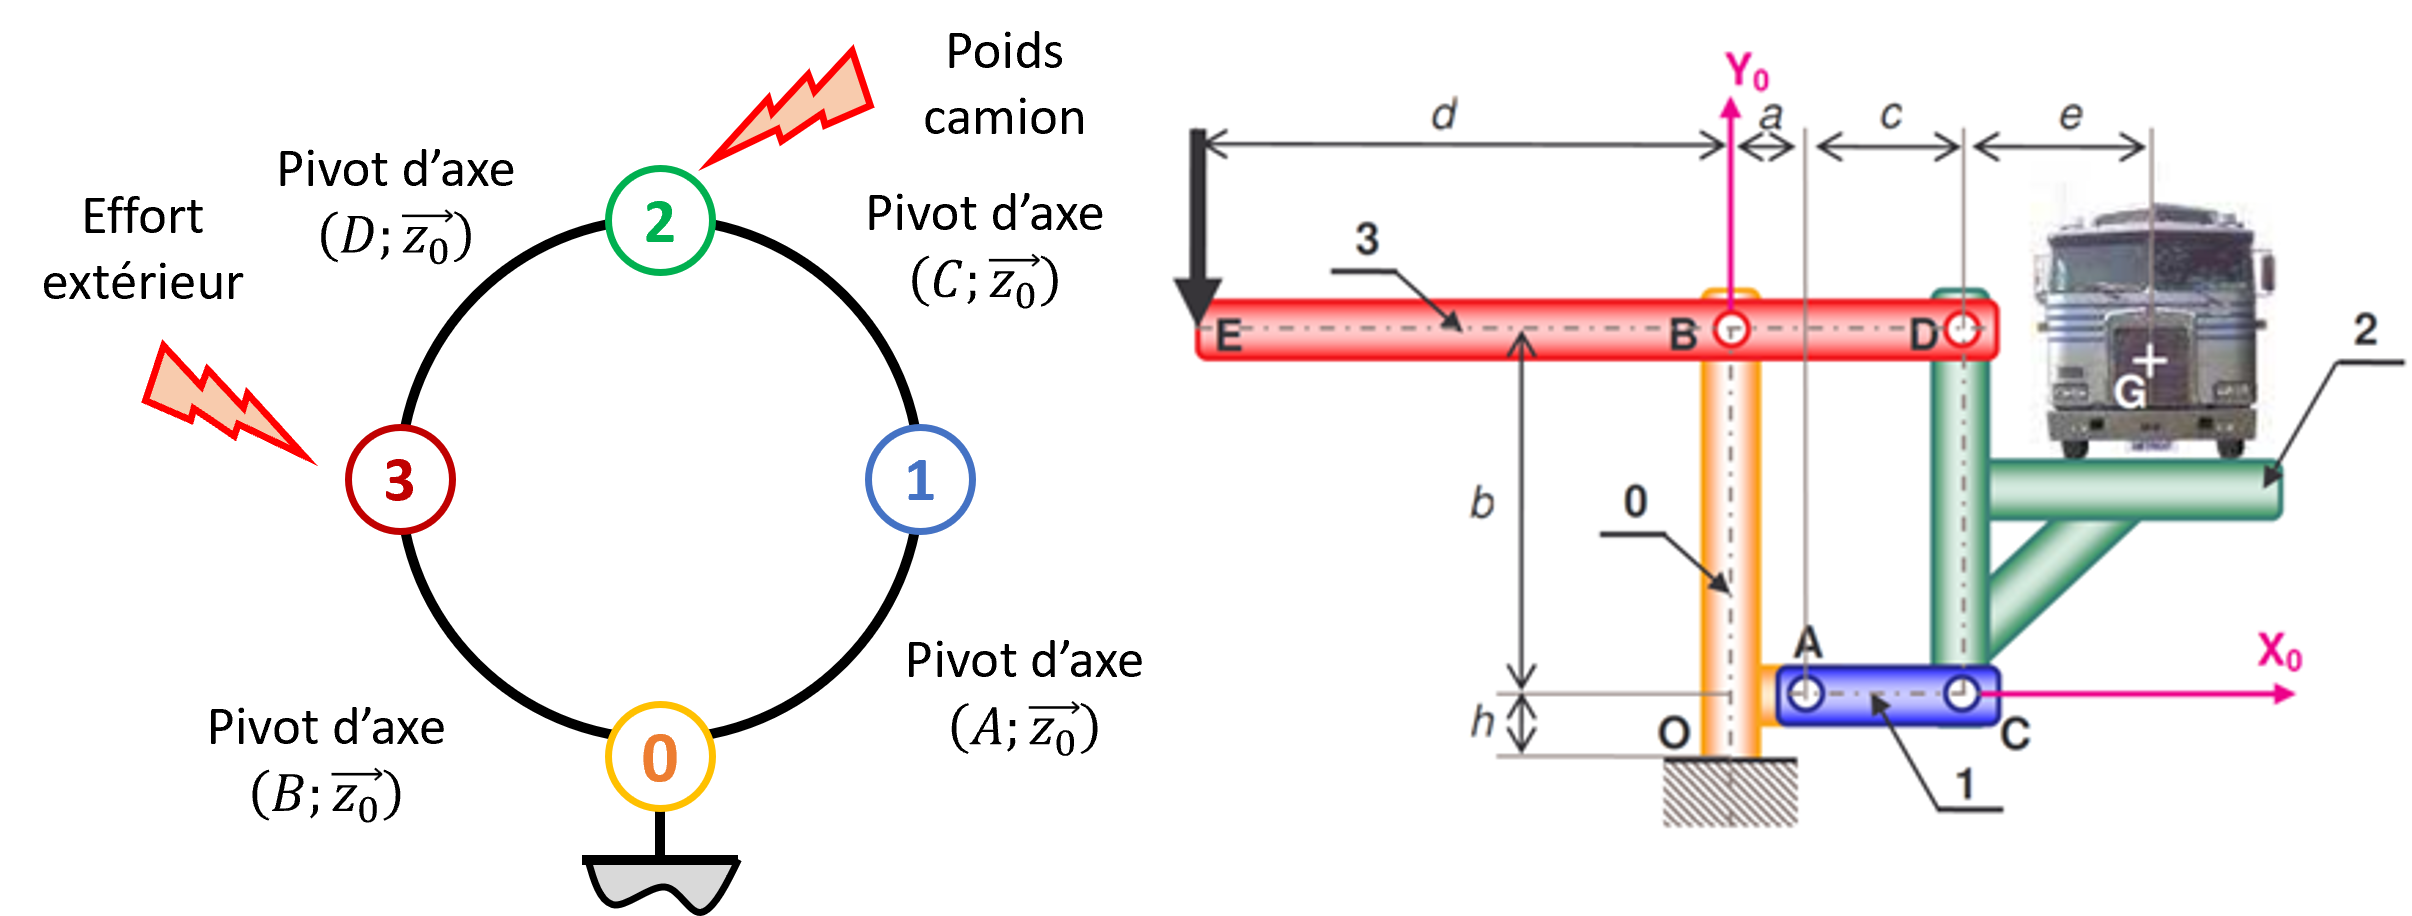
\includegraphics[width=.95\linewidth]{pfs_strategie_pese_camion}
\end{center}
	\begin{reponses}	
	\bonne {le TMS.}
	\mauvaise {le TRS.}
	\mauvaise {le PFS.}
	\mauvaise {en $A$.}
	\bonne {en $B$.}
	\mauvaise {en $C$.}
	\mauvaise {en $D$.}
	\mauvaise {en $E$.}
	\mauvaise {en projection sur $\vx{0}$.}
	\mauvaise {en projection sur $\vy{0}$.}		
	\bonne {en projection sur $\vz{0}$.}
		\mauvaise {ce n'est pas la meilleure idée.}
	\end{reponses}
\end{questionmult}\\}


\element{PFSStrat}{
\begin{questionmult}{pfsstrat 03a}
Soit le modèle suivant. On cherche, en statique, la relation entre le poids et l'effort dans le vérin. Le problème est plan.
\begin{center}
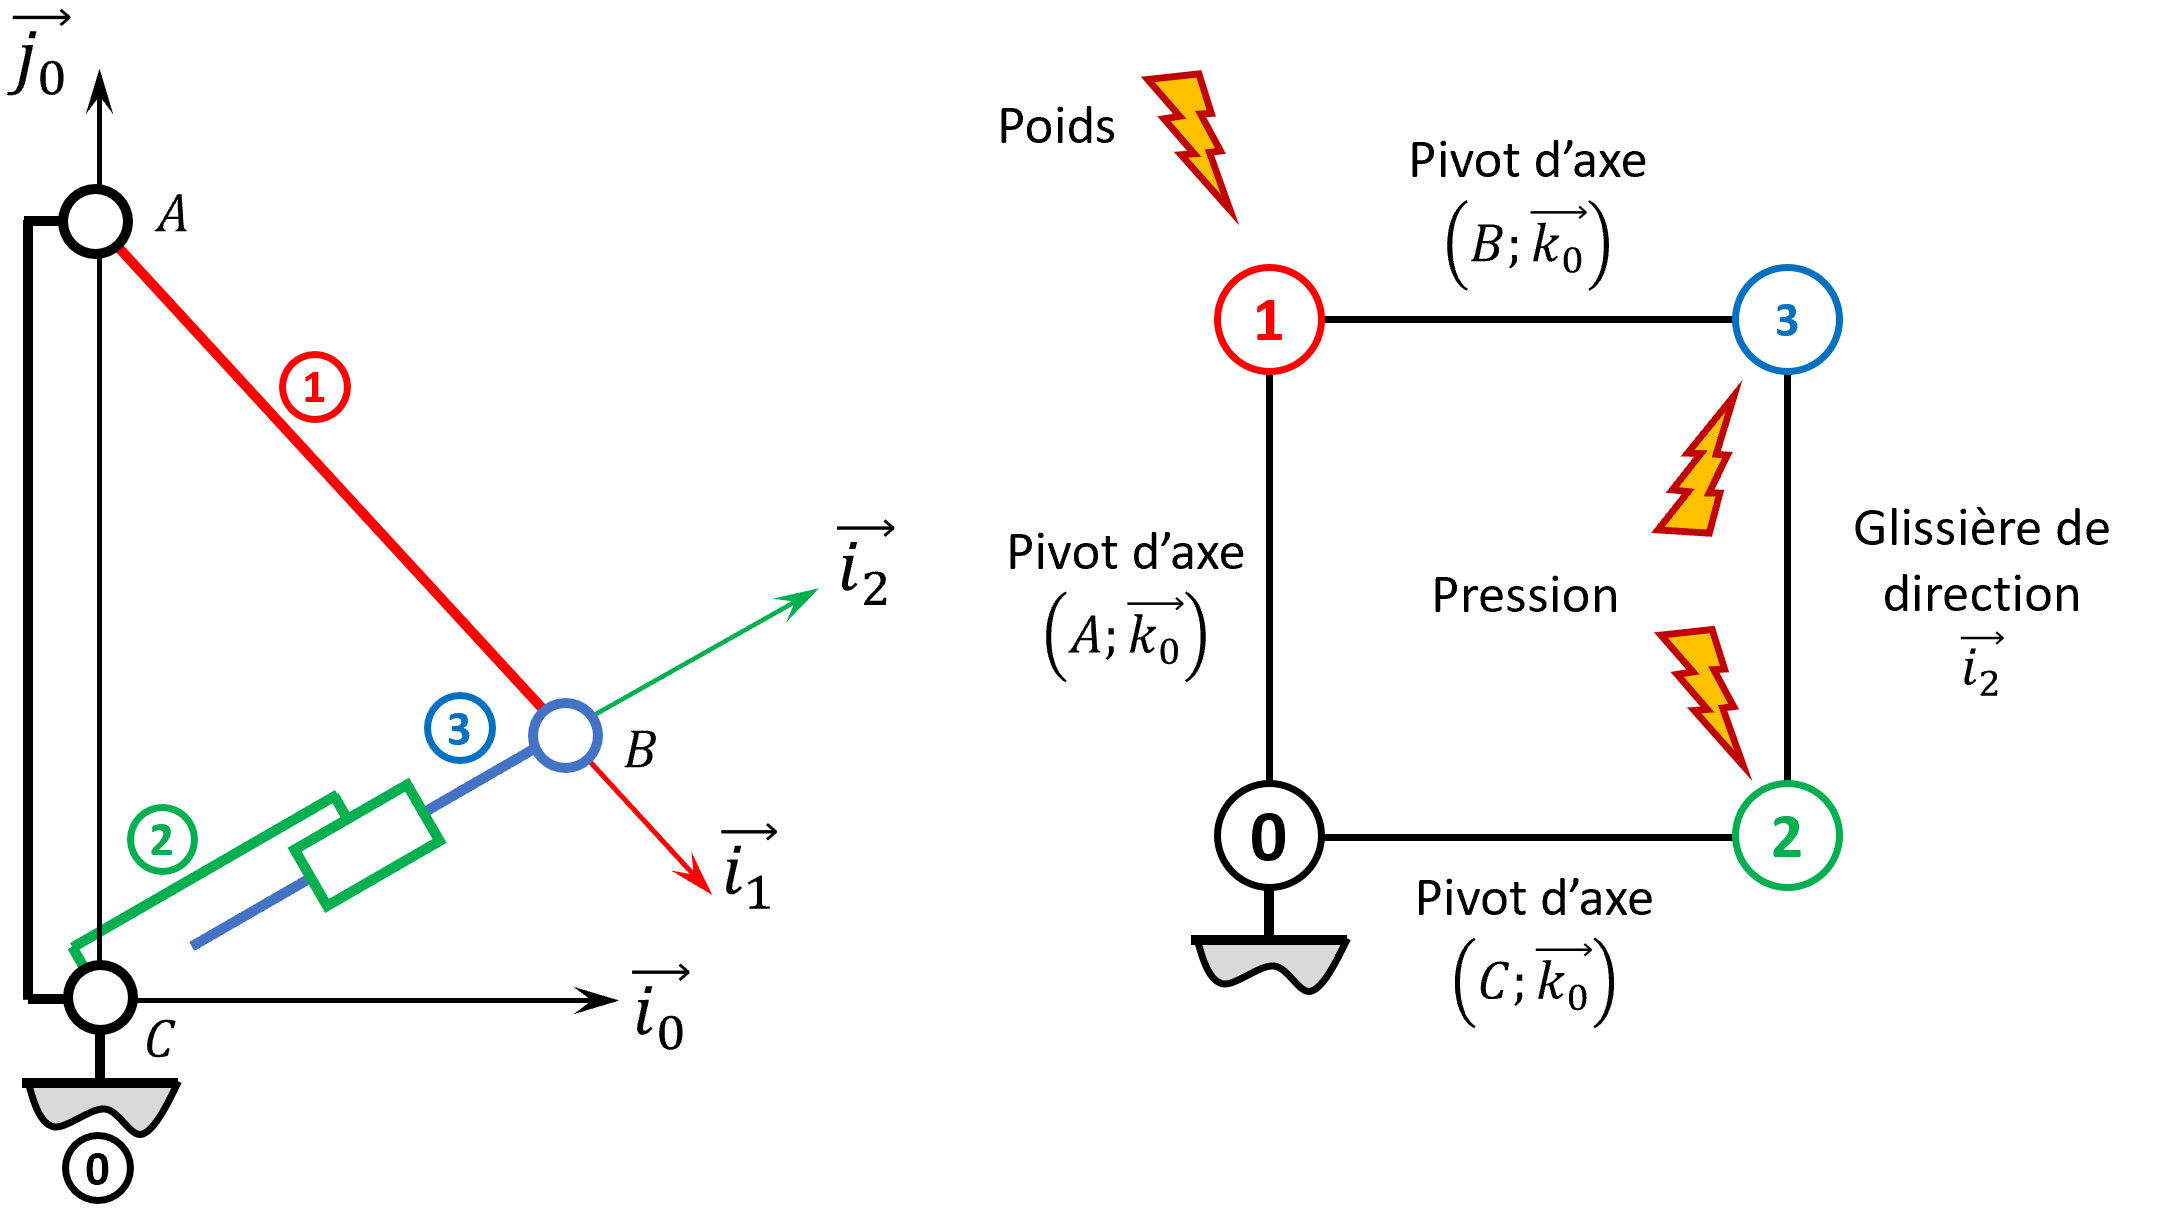
\includegraphics[width=.95\linewidth]{pfs_strategie_verin.png}
\end{center}
	\begin{reponses}	
	\mauvaise{On commence par isoler 1.} 
	\mauvaise {Peu importe.}
	\mauvaise {On commence par isoler 1+2+3.} 
	\mauvaise {On commence par isoler 1+2+3.} 
	\mauvaise {On commence par isoler 1+2.} 
	\bonne {On commence par isoler 3+2.} 
	\mauvaise {On commence par isoler 3+1.} 
	\mauvaise {On commence par isoler 3.}
	\mauvaise {On commence par isoler 0.}
	\end{reponses}
\end{questionmult}\\}

\element{PFSStrat}{
\begin{questionmult}{pfsstrat 03b}
Soit le modèle suivant. On cherche, en statique, la relation entre le poids et l'effort dans le vérin. Le problème est plan.
On a isolé 1. Quelle équation est-il préférable d'écrire ?
\begin{center}
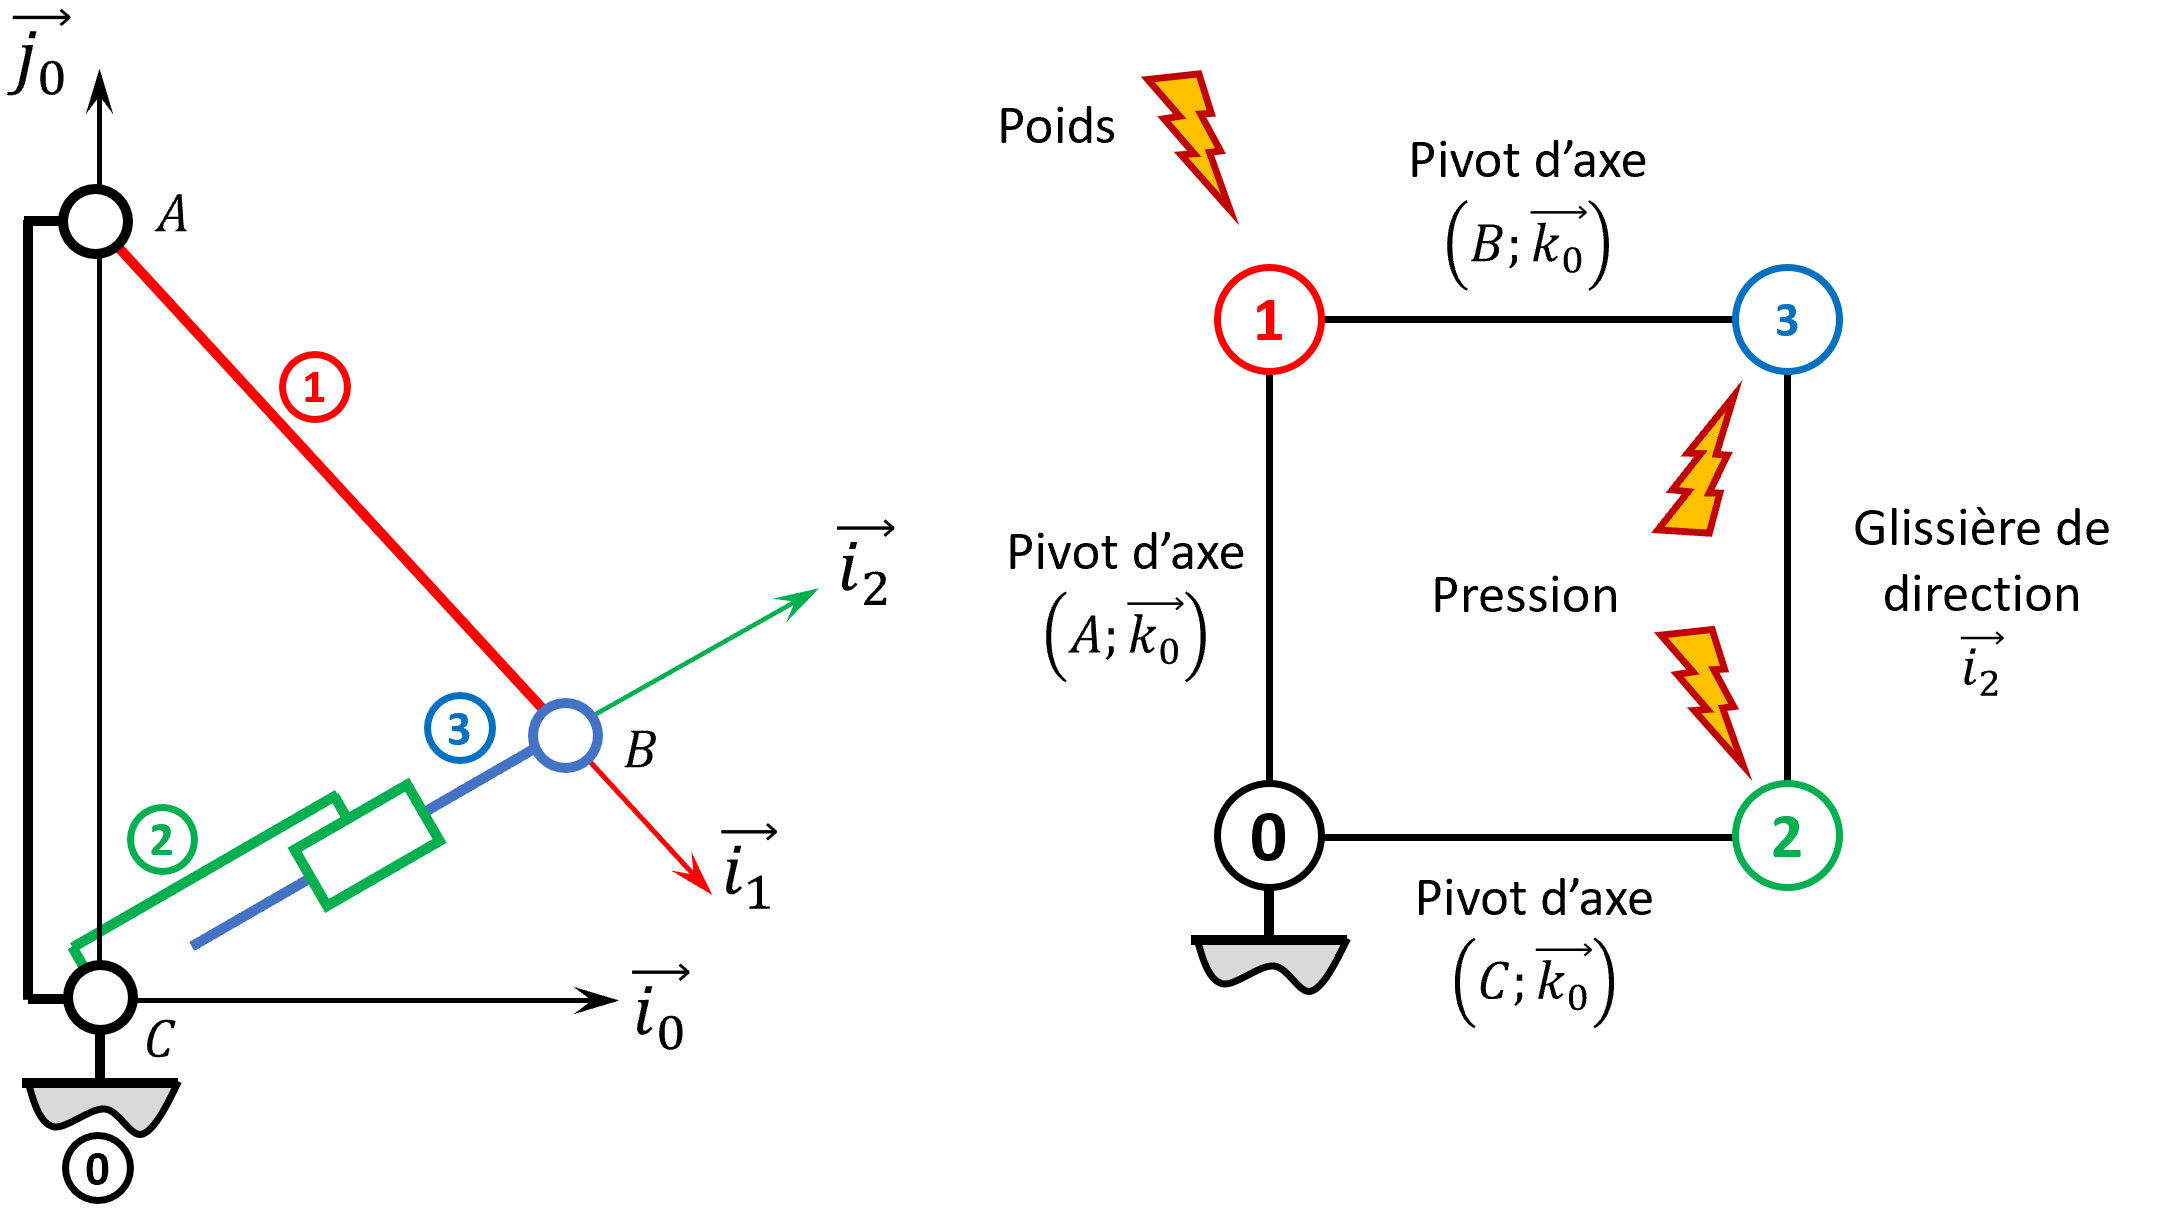
\includegraphics[width=.95\linewidth]{pfs_strategie_verin.png}
\end{center}
	\begin{reponses}	
	\bonne {le TMS.}
	\mauvaise {le TRS.}
	\mauvaise {le PFS.}
	\bonne{en $A$.}
	\mauvaise {en $B$.}
	\mauvaise {en $C$.}
	\mauvaise {ce n'est pas la meilleure idée.}
	\mauvaise {en projection sur $\vi{0}$.}
	\mauvaise {en projection sur $\vj{0}$.}		
	\mauvaise {en projection sur $\vi{1}$.}
	\mauvaise {en projection sur $\vj{1}$.}		
	\mauvaise {en projection sur $\vi{2}$.}
	\mauvaise {en projection sur $\vj{2}$.}		
	\bonne {en projection sur $\vz{0}$.}	
	\end{reponses}
\end{questionmult}\\}

\element{PFSStrat}{
\begin{questionmult}{pfsstrat 03c}
Soit le modèle suivant. On cherche, en statique, la relation entre le poids et l'effort dans le vérin. Le problème est plan.
On a isolé 2. Quelle équation est-il préférable d'écrire ?
\begin{center}
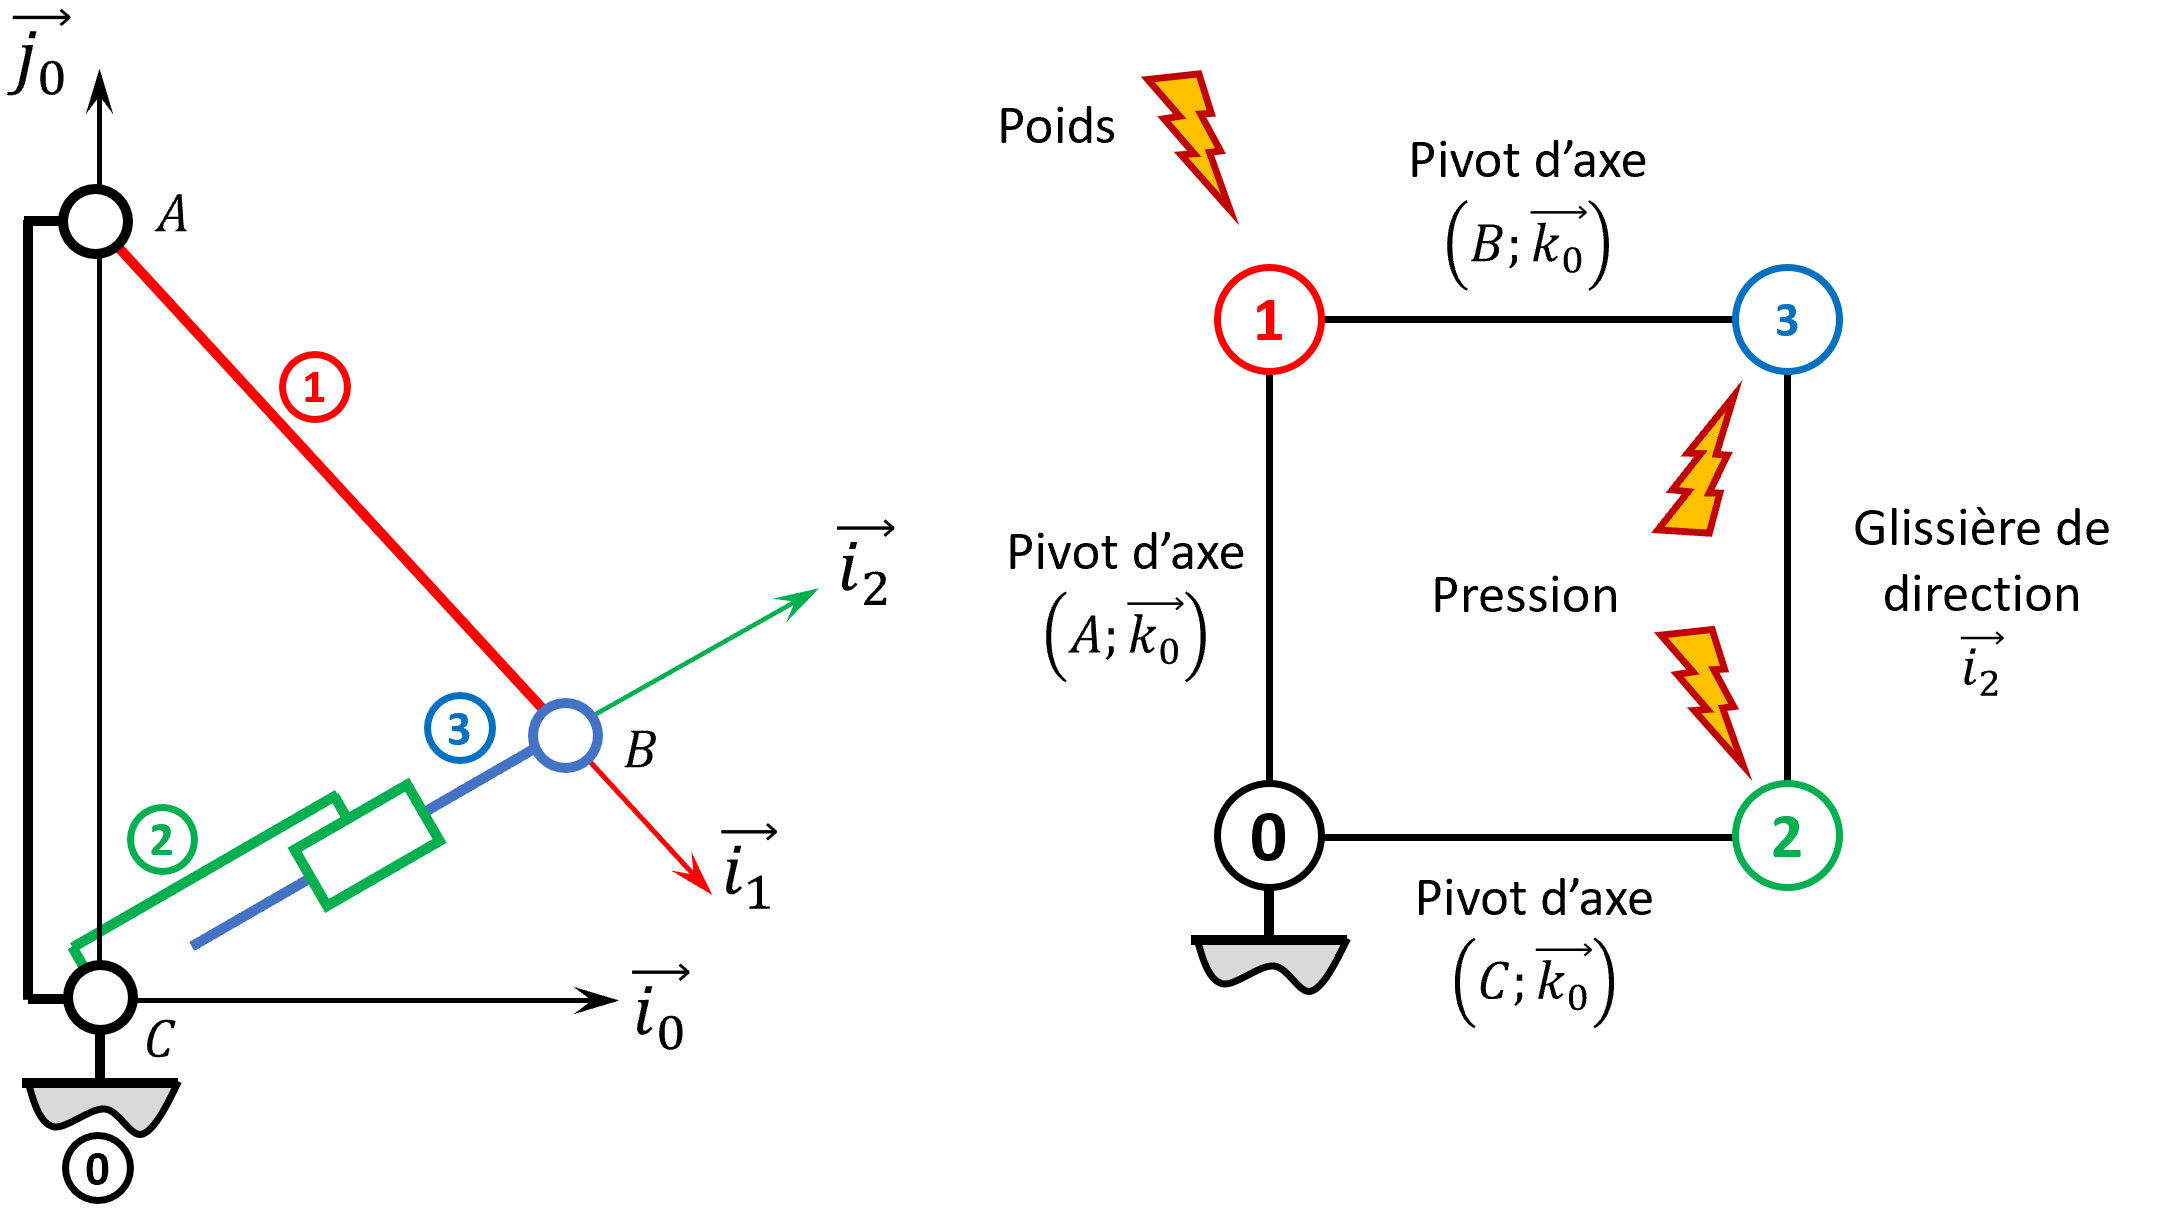
\includegraphics[width=.95\linewidth]{pfs_strategie_verin.png}
\end{center}
	\begin{reponses}	
	\mauvaise {le TMS.}
	\mauvaise {le TRS.}
	\mauvaise {le PFS.}
	\mauvaise {en $A$.}
	\mauvaise {en $B$.}
	\mauvaise {en $C$.}
	\bonne{ce n'est pas la meilleure idée.}
	\mauvaise {en projection sur $\vi{0}$.}
	\mauvaise {en projection sur $\vj{0}$.}		
	\mauvaise {en projection sur $\vi{1}$.}
	\mauvaise {en projection sur $\vj{1}$.}		
	\mauvaise {en projection sur $\vi{2}$.}
	\mauvaise {en projection sur $\vj{2}$.}		
	\mauvaise {en projection sur $\vz{0}$.}	
	\end{reponses}
\end{questionmult}\\}
